% !TEX root = ../../../main.tex
% 来源：中学数学实验教材·第三册（高中数学）
% 章节：三角函数的图象和性质 / 正切函数的图象和性质
% 原始文件：7.tex，行 884-925
% 类型：tikz
% ---
    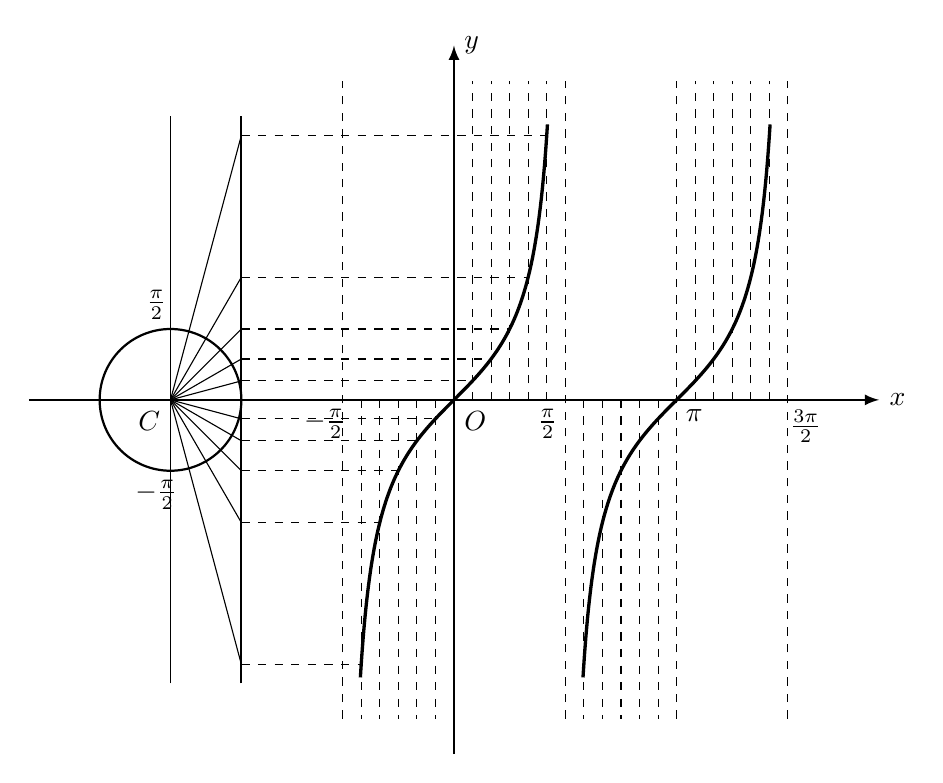
\begin{tikzpicture}[>=latex, scale=.9]
        \draw[->, thick] (-6,0)--(6,0)node[right]{$x$};   
\draw[->, thick] (0,-5)--(0,5)node[right]{$y$};
\draw[thick] (-4,0) circle(1);
\draw (-4,-4)--(-4,4);
\draw[thick] (-3,-4)--(-3,4);
\foreach \x in {-5,-4,...,5}
{
    \draw (-4,0) -- (-3, {tan(\x*pi/12 r)});
}

\foreach \y in {-.5,.5}
{
    \draw [domain=\y*pi+.25:(\y+1)*pi-.25, samples=1000, very thick] plot(\x, {tan(\x r)});
}

\foreach \x in {-5,-4,...,-1,7,8,...,11}
{
    \draw[dashed] (\x*pi/12,0)--(\x*pi/12,-4.5);
}
\foreach \x in {1,2,...,5,13,14,...,17}
{
    \draw[dashed] (\x*pi/12,0)--(\x*pi/12,4.5);
}
\foreach \x in {-1,1,2,3}
{
    \draw [dashed] (\x*pi/2, -4.5)--(\x*pi/2, 4.5);
}

\foreach \x in {-5,-4,...,5}
{
    \draw[dashed] (-3, {tan(\x*pi/12 r)})--(\x*pi/12, {tan(\x*pi/12 r)});
}
\node at (-4.3,-.3){$C$};
\node at (-4.2,1)[above]{$\frac{\pi}{2}$};
\node at (-4.2,-1)[below]{$-\frac{\pi}{2}$};
\node at (.3,-.3){$O$};
\node at (-pi/2-.25,0)[below]{$-\frac{\pi}{2}$};
\node at (pi/2-.25,0)[below]{$\frac{\pi}{2}$};
\node at (3*pi/2+.25,0)[below]{$\frac{3\pi}{2}$};
\node at (pi+.25,0)[below]{$\pi$};
    \end{tikzpicture}
